\subsection{Componenti per il random access e le LCE query}
Le ultime componenti da descrivere sono quelle atte a garantire il
\textit{random access} 
al testo e, nel caso dell'uso degli \textit{SLP}, permettere il computo delle
\textit{LCE query}.\\
Parlando di strutture per il random access una differenza sostanziale tra
l'uso di un \textit{vettore di bitvector}, \texttt{RA-BV}, e quello
dell'\textit{SLP}, \texttt{RA-SLP}, è data dai tempi di accesso ai singoli
elementi. Infatti, parlando di \texttt{RA-BV}, si ha accesso in tempo costante
ad un qualsiasi elemento del pannello mentre, nel caso di \texttt{RA-SLP},
denotando con $s$ la lunghezza della parola generata dall'\textit{SLP}, si ha
che l'accesso ad ogni elemento è in tempo:
\begin{equation}
  \label{eq:timera}
  \mathcal{O}(\log s)
\end{equation}
La seconda differenza, già ampiamente introdotta e di fatto scontata, è data
dalla dimensione delle due strutture dati, avendo che \texttt{RA-BV} memorizza
$\sim NM$ bit, dove il $\sim$ è dato dai costi in memoria aggiuntivi dati
dall'avere un vettore che memorizza i bitvector. Parlando invece di
\texttt{RA-SLP} non si può avere una stima teorica dello spazio necessario ma,
come si vedrà nel capitolo \ref{reschap}, i risultati quantitativi daranno prova
della capacità di compressione degli \textit{SLP}.\\
Parlando della componente \texttt{LCE} bisogna solo descrivere il modo con cui
si ottiene la singola stringa che verrà compressa tramite \textit{SLP}.
In primis, le
librerie per la costruzione di tale struttura assumono un input
``monodimensionale'', ovvero una singola sequenze lineare. Inoltre, anche per
permettere la costruzione efficiente della \textit{PBWT}, e conseguentemente
della \textit{RLPBWT}, il pannello in input risulta essere trasposto, avendo che
le righe nel file in input rappresentano i siti e non gli individui. Bisogna
quindi in primis trasporre tale pannello. Per procedere ulteriormente bisogna
però ricordare che sull'\textit{SLP} si avrà 
necessità di effettuare \textit{LCE query} che però, si anticipa, nel nostro
pannello, devono essere fatte tra due righe da destra a sinistra (a differenza
di quanto visto nel caso standard dove si confrontavano prefissi comuni). Per
rendere possibile questa operazione quindi il pannello deve essere sia 
salvato come un'unica riga, per ottenerne l'\textit{SLP}, che ``da destra a
sinistra'', per permettere le \textit{LCE query}. Si procede quindi concatenando
ogni riga, selezionandole consecutivamente e leggendone i singoli elementi da
destra a sinistra.
\begin{esempio}
  Si vede quindi un breve esempio.\\
  Si assuma di avere il seguente pannello nel file in input.
  \[
    X=\left[
      \begin{matrix}
        0 & 0 & 1 & 0 & 0\\
        1 & 1 & 1 & 0 & 1\\
        0 & 1 & 1 & 1 & 1\\
        0 & 0 & 0 & 1 & 0
      \end{matrix}
    \right]
  \]
  Dove però come detto le righe sono i siti e le colonne i sample. Per ottenere
  l'\textit{SLP} biosgna quindi, in primis, trasporre la matrice:
  \[
    X^T=\left[
      \begin{matrix}
        0 & 1 & 0 & 0\\
        0 & 1 & 1 & 0\\
        1 & 1 & 1 & 0\\
        0 & 0 & 1 & 1\\
        0 & 1 & 1 & 0
      \end{matrix}
    \right]
  \]
  A questo punto bisogna considerare l'ordine in cui si vorranno effettuare le
  \textit{LCE query}.
  Ad esempio, prendendo la seconda e la terza riga, facendo partire il confronto
  dall'ultima colonna, avremmo una \textit{LCE
    query} lunga 3, terminante nella prima colonna esclusa:
  \begin{figure}[H]
    \centering
    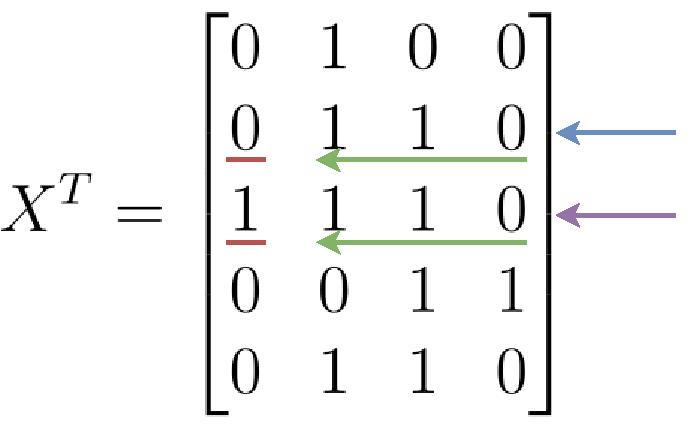
\includegraphics[scale = 0.38]{img/slppanel.pdf}
  \end{figure}
  Si procede quindi salvano la sequenza lineare relativa al pannelli come
  descritto sopra,
  ottenendo, con colorate gli stessi risultati della query fatta
  sopra:
  \[0010\,\,{\color{nordgreen}011}{\color{nordred}0}\,\,
    {\color{nordgreen}011}{\color{nordred}1} \,\,1100\,\,0110\]
  \textit{Si noti che qui si sono segnalate le varie righe con uno spazio ma
    solo per praticità ``visiva''.}
\end{esempio}
In termini di complessità, si ricorda che, come per il \textit{random access},
per il calcolo delle \textit{LCE query} con \textit{SLP} si ha un tempo
proporzionale a: 
\begin{equation}
  \label{eq:timelce}
  \mathcal{O}(\log s)
\end{equation}